\chapter{Appendix}%
\label{ch:appendix}

% Appendix 1
\section{Literature Search and Screening Log}
\label{sec:screening-log}

This appendix documents the structured literature search conducted during Phase~2 of the project. The search was performed across four databases: Google Scholar, ACM Digital Library, IEEE Xplore, and SpringerLink. Search strings were formed by combining topic keywords across the four literature strands of this thesis.

\subsection*{Search Strings}

The following query combinations were used:

\begin{itemize}
  \item \texttt{"explainable AI" AND "decision support"}
  \item \texttt{"explainable AI" AND "interpretability evaluation"}
  \item \texttt{"usable security" AND "security reporting"}
  \item \texttt{"usable security" AND "security dashboards"}
  \item \texttt{"software architecture" AND "abstractions" AND "stakeholders"}
  \item \texttt{"data-to-text" AND "explanation generation"}
  \item \texttt{"data-to-text" AND "technical communication"}
  \item \texttt{"vulnerability management" AND "explainability"}
  \item \texttt{"cybersecurity" AND "non-technical stakeholders" AND "explanation"}
\end{itemize}

\subsection*{Inclusion and Exclusion Criteria}

\begin{table}[h]
\centering
\begin{tabular}{@{}lp{0.75\textwidth}@{}}
\toprule
\textbf{Criterion} & \textbf{Description} \\
\midrule
\textbf{Include} & Peer-reviewed articles, conference papers, or books \\
                 & Directly addresses one of the four literature strands \\
                 & Published in English \\
                 & Relevant to stakeholder-oriented explanation, XAI methods, SE architecture, usable security, or data-to-text \\
\midrule
\textbf{Exclude} & Grey literature (blog posts, vendor white papers) unless no academic equivalent exists \\
                 & Purely algorithmic ML papers with no discussion of human interpretation \\
                 & Papers focused on detection performance only, without explanation component \\
                 & Duplicate or highly similar coverage already provided by a survey paper \\
\bottomrule
\end{tabular}
\caption{Inclusion and exclusion criteria for literature screening.}
\label{tab:screening-criteria}
\end{table}

\subsection*{Screening Results by Strand}

\begin{table}[h]
\centering
\begin{tabular}{@{}lp{0.45\textwidth}rr@{}}
\toprule
\textbf{Strand} & \textbf{Key Sources} & \textbf{Screened} & \textbf{Retained} \\
\midrule
XAI and Human-Centred Explanation
  & Barredo Arrieta et al.~\cite{barredo2020xai}; Guidotti et al.~\cite{guidotti2018survey}; Miller~\cite{miller2019explanation}; Doshi-Velez \& Kim~\cite{doshivelez2017rigorous}; Lipton~\cite{lipton2018mythos}; Liao et al.~\cite{liao2020questioning}; Ribeiro et al.~\cite{ribeiro2016should}; Lundberg \& Lee~\cite{lundberg2017unified}; Wachter et al.~\cite{wachter2017counterfactual}
  & 42 & 9 \\
\midrule
Software Architecture and Abstraction
  & Bass et al.~\cite{bass2012software}; Parnas~\cite{parnas1972modules}; Kruchten~\cite{kruchten1995viewmodel}
  & 28 & 3 \\
\midrule
Usable Security and Security Communication
  & Cranor~\cite{cranor2008framework}; Werlinger et al.~\cite{werlinger2008ids}
  & 31 & 2 \\
\midrule
Data-to-Text and NLG
  & Reiter \& Dale~\cite{reiter2000nlg}; Gatt \& Krahmer~\cite{gatt2018survey}
  & 19 & 2 \\
\midrule
\textbf{Total} & & \textbf{120} & \textbf{15} \\
\bottomrule
\end{tabular}
\caption{Summary of literature screening results by strand.}
\label{tab:screening-results}
\end{table}

Selection proceeded in three steps: (1)~title and abstract screening against the inclusion criteria; (2)~full-text screening for relevance to stakeholder-oriented explanation or software integration; and (3)~backward and forward snowballing from highly relevant survey papers. Priority was given to survey papers and seminal works to establish broad coverage without bias toward any single technique.

% Appendix 2
\section{Design Principles to Architecture Layer Mapping}
\label{sec:dp-mapping}

\Cref{tab:dp-mapping} summarises how each design principle derived from the literature maps to a layer in the four-layer architecture proposed in this thesis.

\begin{table}[h]
\centering
\begin{tabular}{@{}llp{0.45\textwidth}@{}}
\toprule
\textbf{Principle} & \textbf{Architecture Layer} & \textbf{Architectural Implication} \\
\midrule
DP1 — Audience-relative explanation   & Stakeholder View    & Separate renderers for technical and non-technical roles; role is an explicit input parameter \\
DP2 — Selective and contrastive content & Explanation         & Ranking logic selects top contributing factors; contrastive note generated when multiple vulnerabilities are compared \\
DP3 — Evidence traceability           & Explanation + Ingestion & Each explanation object carries pointers back to the source scanner fields that drove it \\
DP4 — Separation of explanation concerns & All layers         & Parsing, abstraction, explanation logic, and view rendering are implemented as independent components with defined interfaces \\
DP5 — Stakeholder-oriented abstraction layers & Abstraction    & Raw scanner fields are mapped to abstract concepts (e.g.\ exploit likelihood, business impact) before explanation generation \\
DP6 — Translation as a design problem & Explanation         & Explanation objects are produced through content selection, factor aggregation, and template-based realisation \\
DP7 — Modifiability for evolving toolchains & Ingestion       & The parser is isolated behind a normalised internal representation; swapping the data source does not affect downstream layers \\
DP8 — Human interpretation over completeness & Stakeholder View & Non-technical views suppress raw scores in favour of plain-language risk summaries; uncertainty is surfaced explicitly \\
\bottomrule
\end{tabular}
\caption{Mapping of design principles to architecture layers.}
\label{tab:dp-mapping}
\end{table}

% Appendix 3 — Phase 1 Interview Data
\section{Phase 1 Interview Data}
\label{sec:interview-data}

This appendix documents the data collected during Phase~1 of the research. It includes a participant overview, the interview questions used, and a summary of coded responses per participant. All participants are identified by codes to preserve anonymity. Responses are summarised and paraphrased; no verbatim quotes are used. Additional participants may be added before final submission.

% ─────────────────────────────────────────────
\subsection*{Participant Overview}
% ─────────────────────────────────────────────

\begin{table}[h]
\centering
\begin{tabular}{@{}lllll@{}}
\toprule
\textbf{Code} & \textbf{Role} & \textbf{Stakeholder Group} & \textbf{Question Set} & \textbf{Status} \\
\midrule
P1 & Security Transformation Senior Manager  & Non-technical & Standard (Q1--Q5) & Completed \\
P2 & Security Transformation Senior Analyst  & Non-technical & Standard (Q1--Q5) & Completed \\
P3 & Security (non-operational)              & Expert informant & Validation (V1--V4) & Completed \\
P4 & Security Transformation Analyst         & Non-technical & Standard (Q1--Q5) & Completed \\
P5 & [Technical role -- TBD]                 & Technical     & Standard (Q1--Q5) & Pending \\
\bottomrule
\end{tabular}
\caption{Overview of Phase~1 interview participants.}
\label{tab:participants}
\end{table}

P3 indicated at the outset that they no longer perform operational vulnerability management and answered a set of targeted validation questions rather than the standard interview guide. Their responses are used to validate specific design decisions rather than to elicit new requirements. P3 also referred the researcher to a red team lead for contact with technical practitioners; that contact is being pursued and will be documented as P5 if an interview is completed.

% ─────────────────────────────────────────────
\subsection*{Interview Questions}
% ─────────────────────────────────────────────

\paragraph{Standard question set (P1, P2, P4).}

\begin{enumerate}
  \item What decisions do you typically make when vulnerability findings come your way? What information do you actually need to act on them?
  \item Which parts of current security reports or outputs are unclear or not useful for your role?
  \item What would an ideal explanation of a vulnerability finding look like? What should it contain to be useful for you or your clients?
  \item What would make you trust -- or not trust -- an explanation coming from an automated tool?
  \item When communicating findings to clients or senior stakeholders, what makes that conversation easy or difficult?
\end{enumerate}

\paragraph{Validation question set (P3).}

\begin{enumerate}[label=V\arabic*.]
  \item How do you currently bridge the gap between raw security data and what you or your client need to understand? What effort does that cost you?
  \item If a tool automatically generated a summary of a vulnerability finding, what would you need in order to trust it?
  \item If immediate patching is not possible, would it help if the explanation also proposed temporary mitigating measures?
  \item How specific would a recommended action need to be in order to be useful?
\end{enumerate}

% ─────────────────────────────────────────────
\subsection*{Coded Responses by Participant}
% ─────────────────────────────────────────────

Responses were coded using a lightweight thematic analysis approach. The goal was requirement extraction rather than sociological theory-building. Each response is summarised against the relevant question set.

\paragraph{P1 -- Security Transformation Senior Manager}

\begin{table}[h]
\centering
\begin{tabular}{@{}lp{0.72\textwidth}@{}}
\toprule
\textbf{Question} & \textbf{Summary} \\
\midrule
Q1 & The primary decision is the trade-off between patching priority and the operational impact of patching on the affected system or service. Required information includes: where the vulnerability is located, how to resolve it, the risk relative to actual system exposure (not just the vulnerability in isolation), and any mitigating measures that can be applied until patching is possible. \\
\midrule
Q2 & Current tool outputs are often unclear about where exactly the vulnerability was found and, more critically, about how much risk the system actually faces in its specific environment. \\
\midrule
Q3 & An ideal explanation would include context-specific risk information that reflects the actual exposure of the system, not a generic severity statement. \\
\midrule
Q4 & Trust increases when information is recognisably specific and relevant to the actual environment and context. Trust decreases rapidly when outputs are generic or repeatedly inaccurate. \\
\midrule
Q5 & The most important factor in client conversations is the ability to explain why a finding has a particular priority. When clients resist patching due to operational impact, the conversation requires acknowledging that concern while still conveying the risk clearly enough to justify action or the adoption of temporary mitigating measures. \\
\bottomrule
\end{tabular}
\caption{Coded responses for P1.}
\label{tab:p1-responses}
\end{table}

\paragraph{P2 -- Security Transformation Senior Analyst}

\begin{table}[h]
\centering
\begin{tabular}{@{}lp{0.72\textwidth}@{}}
\toprule
\textbf{Question} & \textbf{Summary} \\
\midrule
Q1 & Proper prioritisation is the foundation for acting on findings. Key inputs include: a complete picture of affected assets and their exposure breadth, a justification for the scoring rather than the score alone, exploitability status (known exploits should raise priority), and available fixes or workarounds for cases where no patch exists. \\
\midrule
Q2 & The scoring-severity relationship is sometimes confusing, particularly when a high \ac{CVSS} score does not correspond to the expected severity level. More fundamentally, context and network structure are not embedded in the scoring: the same vulnerability on an air-gapped server and on an internet-exposed server receives the same score, which is not meaningful for prioritisation decisions. \\
\midrule
Q3 & A useful format would include at minimum: vulnerability name, short description, \ac{CVE} identifier, \ac{CVSS} score, severity, number or list of affected assets, exploitability level, known exploits, and possible fixes. Context analysis is essential for the explanation to be trustworthy. \\
\midrule
Q4 & Trust requires the ability to justify the severity and score from the explanation provided. Reports need to be up to date, thorough, and readable. A report that cannot explain the reasoning behind its scores loses credibility quickly. \\
\midrule
Q5 & In a previous engagement, the participant created a custom report after a scanning exercise because the tool's out-of-the-box output lacked sufficient context, requiring additional independent research. A further simplified version was produced for non-technical stakeholders, translating findings into business impact terms and explaining prioritisation choices. This translation process was described as challenging. \\
\bottomrule
\end{tabular}
\caption{Coded responses for P2.}
\label{tab:p2-responses}
\end{table}

\paragraph{P3 -- Security (non-operational), Expert Informant}

\begin{table}[h]
\centering
\begin{tabular}{@{}lp{0.72\textwidth}@{}}
\toprule
\textbf{Question} & \textbf{Summary} \\
\midrule
V1 & Bridging the gap between raw data and actionable insight depends heavily on contextual knowledge of the systems and the environment. Without that knowledge, assessing actual impact is difficult. This suggests that any automated system must embed context rather than expecting the reader to supply it. \\
\midrule
V2 & Trust in an automated summary depends on whether the sources and evidence are applicable to the client's specific systems. Generic outputs based on non-applicable sources are not trustworthy. \\
\midrule
V3 & Temporary mitigating measures are considered important when patching is not immediately possible. However, mitigations carry their own trade-offs and disadvantages, which should be weighed and communicated alongside the mitigation itself. \\
\midrule
V4 & Recommended actions must be highly specific. An incorrect mitigation applied to the wrong system or vulnerability can cause damage. Actions must be validated against the exact system and vulnerability in scope. \\
\bottomrule
\end{tabular}
\caption{Coded responses for P3 (validation question set).}
\label{tab:p3-responses}
\end{table}

\paragraph{P4 -- Security Transformation Analyst}

\begin{table}[h]
\centering
\begin{tabular}{@{}lp{0.72\textwidth}@{}}
\toprule
\textbf{Question} & \textbf{Summary} \\
\midrule
Q1 & Acting on a finding requires first establishing whether it is a genuine finding (false positives are encountered regularly) and then determining urgency, asset ownership, and required action. The decision is not binary; it involves choosing between immediate remediation, further validation, owner clarification, risk acceptance, or escalation. Required information includes: affected asset, severity, business service supported by the asset, responsible owner, remediation action, SLA or deadline, and expected operational impact such as reboots or downtime. \\
\midrule
Q2 & Current reports often provide the \ac{CVE} identifier, severity, and affected system but fail to clarify who should act, what business service is affected, whether the system is in production, and what the remediation impact will be. Prioritisation is also difficult when there are many findings and severity alone does not distinguish a critical finding on an internet-facing production system from the same finding on an isolated test system. \\
\midrule
Q3 & A useful explanation should be short, structured, and role-adapted. Suggested fields: summary, affected asset and service, risk expressed in plain terms, required action, responsible owner, urgency or deadline, and operational impact of the remediation. Technical teams require more detail; management requires business impact framing and clear decision points. \\
\midrule
Q4 & Trust in a tool-generated explanation increases when it is traceable to the original scanner finding and shows the key evidence behind the summary. The explanation should clearly separate facts from assumptions and should not claim to know asset ownership, business impact, SLA exceptions, or final remediation decisions. Distrust arises when the explanation sounds confident without supporting evidence, oversimplifies the finding, or recommends actions that have not been operationally validated. \\
\midrule
Q5 & Communication is straightforward when the finding includes clear risk, impact, owner, and required action. It becomes difficult when the message is too technical, when ownership is unclear, or when the explanation does not address what each stakeholder specifically needs to do. \\
\bottomrule
\end{tabular}
\caption{Coded responses for P4.}
\label{tab:p4-responses}
\end{table}

% ─────────────────────────────────────────────
\subsection*{Thematic Summary}
\label{subsec:thematic-summary}
% ─────────────────────────────────────────────

Eight recurring themes were identified across the completed responses. Table~\ref{tab:themes} summarises each theme, the participants who raised it, and the design decision it informed.

\begin{table}[h]
\centering
\begin{tabular}{@{}lp{0.33\textwidth}lp{0.22\textwidth}@{}}
\toprule
\textbf{Theme} & \textbf{Description} & \textbf{Participants} & \textbf{Design Decision} \\
\midrule
T1 & Prioritisation is the primary decision; findings must be ordered and justified & P1, P2, P4 & \texttt{urgency} field; \texttt{top\_factors} ranking \\
\midrule
T2 & Scoring must account for asset context and exposure, not just vulnerability severity in isolation & P1, P2, P4 & Abstraction layer rule tables combining \ac{CVSS} with asset context \\
\midrule
T3 & Exploitability status is a key prioritisation input; known exploits warrant higher priority & P2, P4 & \texttt{exploit\_available} and \texttt{known\_exploited} fields \\
\midrule
T4 & Trust requires traceable justification; generic or overconfident outputs are not trusted & P1, P2, P3, P4 & \texttt{evidence\_pointers}; \texttt{certainty\_level}; \texttt{limitations} field \\
\midrule
T5 & Current tools require practitioners to perform additional manual translation; the gap is real and costly & P1, P2, P4 & Thesis problem statement; non-technical view design \\
\midrule
T6 & Non-technical stakeholders require business impact framing, not technical severity scores & P2, P4 & Non-technical renderer; \texttt{business\_consequence} field \\
\midrule
T7 & False positives are a known concern; a finding must be validated before action is taken & P4 & \texttt{certainty\_level}; \texttt{limitations} field; system should separate facts from assumptions \\
\midrule
T8 & Asset ownership and accountability must be explicit; unclear ownership blocks action & P4 & Acknowledged as scope limitation; asset owner field deferred to future work \\
\bottomrule
\end{tabular}
\caption{Recurring themes from Phase~1 interviews and their mapping to design decisions.}
\label{tab:themes}
\end{table}

Four additional requirements were identified that were not fully anticipated in the initial design. These are documented below and addressed either through a minor schema addition or scoped to future work.

\begin{description}
  \item[R-new-1: Mitigating measures (P1, P3).] Both P1 and P3 identified the need for temporary mitigating measures when patching is not operationally feasible. P3 added that mitigations carry their own trade-offs, which should also be communicated. This is addressed by adding an optional \texttt{mitigation} field to the explanation object, populated when urgency is Immediate but operational constraints may prevent immediate patching.

  \item[R-new-2: Asset exposure breadth (P2).] P2 noted that the number of affected assets influences prioritisation. The current prototype handles single-asset findings. Aggregation across multiple affected assets is identified as a direction for future work.

  \item[R-new-3: Patching operational impact (P1, P4).] Both P1 and P4 raised the operational cost of patching as a factor. The action field templates are extended to acknowledge this where relevant, for example by noting when a patch requires a maintenance window or service restart.

  \item[R-new-4: Asset ownership (P4).] P4 identified asset ownership as essential for acting on a finding; without knowing who is responsible, findings cannot be routed for remediation. The current system does not claim to determine ownership, which is consistent with P4's requirement that a tool should not guess ownership or business accountability. This is acknowledged in the \texttt{limitations} field and deferred as future work.
\end{description}

\section{Decision Tables}
\label{sec:decision-tables}

The three decision trees of the abstraction layer (\cref{sec:abstraction-layer}) are enumerated exhaustively below as decision tables. Each row is one combination of decision-point values and the outcome the tree returns for it. A value of \emph{none} denotes an absent input. The tables were generated directly from the prototype and verified for completeness and consistency: every combination maps to exactly one outcome, and the number of rows equals the product of the decision-point value counts, namely 27, 108, and 72.

\subsection{Exploitation Likelihood}
\begin{longtable}{@{}llll@{}}
\caption{Exploitation likelihood decision table.}\label{tab:dt-likelihood}\\
\toprule
Exploit available & Known exploited & Internet-facing & Outcome \\ \midrule
\endfirsthead
\toprule Exploit available & Known exploited & Internet-facing & Outcome \\ \midrule
\endhead
\bottomrule
\endfoot
True & True & True & High \\
True & True & False & High \\
True & True & none & High \\
True & False & True & High \\
True & False & False & Medium \\
True & False & none & Medium \\
True & none & True & High \\
True & none & False & Medium \\
True & none & none & Medium \\
False & True & True & Medium \\
False & True & False & Medium \\
False & True & none & Medium \\
False & False & True & Low \\
False & False & False & Low \\
False & False & none & Low \\
False & none & True & Low \\
False & none & False & Low \\
False & none & none & Low \\
none & True & True & Unknown \\
none & True & False & Unknown \\
none & True & none & Unknown \\
none & False & True & Unknown \\
none & False & False & Unknown \\
none & False & none & Unknown \\
none & none & True & Unknown \\
none & none & False & Unknown \\
none & none & none & Unknown \\
\end{longtable}

\subsection{Impact}
\begin{longtable}{@{}lllll@{}}
\caption{Impact decision table.}\label{tab:dt-impact}\\
\toprule
Environment & Severity tier & Business-critical & Owner privileged & Outcome \\ \midrule
\endfirsthead
\toprule Environment & Severity tier & Business-critical & Owner privileged & Outcome \\ \midrule
\endhead
\bottomrule
\endfoot
production & high & True & True & Critical \\
production & high & True & False & Critical \\
production & high & True & none & Critical \\
production & high & False & True & Critical \\
production & high & False & False & High \\
production & high & False & none & High \\
production & high & none & True & High \\
production & high & none & False & High \\
production & high & none & none & High \\
production & moderate & True & True & High \\
production & moderate & True & False & High \\
production & moderate & True & none & High \\
production & moderate & False & True & High \\
production & moderate & False & False & Medium \\
production & moderate & False & none & Medium \\
production & moderate & none & True & Medium \\
production & moderate & none & False & Medium \\
production & moderate & none & none & Medium \\
production & low & True & True & Medium \\
production & low & True & False & Medium \\
production & low & True & none & Medium \\
production & low & False & True & Medium \\
production & low & False & False & Low \\
production & low & False & none & Low \\
production & low & none & True & Low \\
production & low & none & False & Low \\
production & low & none & none & Low \\
production & none & True & True & Unknown \\
production & none & True & False & Unknown \\
production & none & True & none & Unknown \\
production & none & False & True & Unknown \\
production & none & False & False & Unknown \\
production & none & False & none & Unknown \\
production & none & none & True & Unknown \\
production & none & none & False & Unknown \\
production & none & none & none & Unknown \\
staging & high & True & True & High \\
staging & high & True & False & High \\
staging & high & True & none & High \\
staging & high & False & True & High \\
staging & high & False & False & Medium \\
staging & high & False & none & Medium \\
staging & high & none & True & Medium \\
staging & high & none & False & Medium \\
staging & high & none & none & Medium \\
staging & moderate & True & True & Medium \\
staging & moderate & True & False & Medium \\
staging & moderate & True & none & Medium \\
staging & moderate & False & True & Medium \\
staging & moderate & False & False & Low \\
staging & moderate & False & none & Low \\
staging & moderate & none & True & Low \\
staging & moderate & none & False & Low \\
staging & moderate & none & none & Low \\
staging & low & True & True & Low \\
staging & low & True & False & Low \\
staging & low & True & none & Low \\
staging & low & False & True & Low \\
staging & low & False & False & Low \\
staging & low & False & none & Low \\
staging & low & none & True & Low \\
staging & low & none & False & Low \\
staging & low & none & none & Low \\
staging & none & True & True & Unknown \\
staging & none & True & False & Unknown \\
staging & none & True & none & Unknown \\
staging & none & False & True & Unknown \\
staging & none & False & False & Unknown \\
staging & none & False & none & Unknown \\
staging & none & none & True & Unknown \\
staging & none & none & False & Unknown \\
staging & none & none & none & Unknown \\
none & high & True & True & Unknown \\
none & high & True & False & Unknown \\
none & high & True & none & Unknown \\
none & high & False & True & Unknown \\
none & high & False & False & Unknown \\
none & high & False & none & Unknown \\
none & high & none & True & Unknown \\
none & high & none & False & Unknown \\
none & high & none & none & Unknown \\
none & moderate & True & True & Unknown \\
none & moderate & True & False & Unknown \\
none & moderate & True & none & Unknown \\
none & moderate & False & True & Unknown \\
none & moderate & False & False & Unknown \\
none & moderate & False & none & Unknown \\
none & moderate & none & True & Unknown \\
none & moderate & none & False & Unknown \\
none & moderate & none & none & Unknown \\
none & low & True & True & Unknown \\
none & low & True & False & Unknown \\
none & low & True & none & Unknown \\
none & low & False & True & Unknown \\
none & low & False & False & Unknown \\
none & low & False & none & Unknown \\
none & low & none & True & Unknown \\
none & low & none & False & Unknown \\
none & low & none & none & Unknown \\
none & none & True & True & Unknown \\
none & none & True & False & Unknown \\
none & none & True & none & Unknown \\
none & none & False & True & Unknown \\
none & none & False & False & Unknown \\
none & none & False & none & Unknown \\
none & none & none & True & Unknown \\
none & none & none & False & Unknown \\
none & none & none & none & Unknown \\
\end{longtable}

\subsection{Urgency}
\begin{longtable}{@{}lllll@{}}
\caption{Urgency decision table.}\label{tab:dt-urgency}\\
\toprule
Likelihood & Patch available & Overdue & Internet-facing & Outcome \\ \midrule
\endfirsthead
\toprule Likelihood & Patch available & Overdue & Internet-facing & Outcome \\ \midrule
\endhead
\bottomrule
\endfoot
High & True & True & True & Immediate \\
High & True & True & False & Immediate \\
High & True & True & none & Immediate \\
High & True & False & True & Immediate \\
High & True & False & False & Immediate \\
High & True & False & none & Immediate \\
High & False & True & True & Immediate \\
High & False & True & False & Immediate \\
High & False & True & none & Immediate \\
High & False & False & True & Immediate \\
High & False & False & False & Immediate \\
High & False & False & none & Immediate \\
High & none & True & True & Immediate \\
High & none & True & False & Immediate \\
High & none & True & none & Immediate \\
High & none & False & True & Immediate \\
High & none & False & False & Immediate \\
High & none & False & none & Immediate \\
Medium & True & True & True & Immediate \\
Medium & True & True & False & Immediate \\
Medium & True & True & none & Immediate \\
Medium & True & False & True & Scheduled \\
Medium & True & False & False & Scheduled \\
Medium & True & False & none & Scheduled \\
Medium & False & True & True & Scheduled \\
Medium & False & True & False & Scheduled \\
Medium & False & True & none & Scheduled \\
Medium & False & False & True & Scheduled \\
Medium & False & False & False & Scheduled \\
Medium & False & False & none & Scheduled \\
Medium & none & True & True & Scheduled \\
Medium & none & True & False & Scheduled \\
Medium & none & True & none & Scheduled \\
Medium & none & False & True & Scheduled \\
Medium & none & False & False & Scheduled \\
Medium & none & False & none & Scheduled \\
Low & True & True & True & Scheduled \\
Low & True & True & False & Scheduled \\
Low & True & True & none & Scheduled \\
Low & True & False & True & Monitor \\
Low & True & False & False & Monitor \\
Low & True & False & none & Monitor \\
Low & False & True & True & Monitor \\
Low & False & True & False & Monitor \\
Low & False & True & none & Monitor \\
Low & False & False & True & Monitor \\
Low & False & False & False & Monitor \\
Low & False & False & none & Monitor \\
Low & none & True & True & Monitor \\
Low & none & True & False & Monitor \\
Low & none & True & none & Monitor \\
Low & none & False & True & Monitor \\
Low & none & False & False & Monitor \\
Low & none & False & none & Monitor \\
Unknown & True & True & True & Immediate \\
Unknown & True & True & False & Scheduled \\
Unknown & True & True & none & Scheduled \\
Unknown & True & False & True & Scheduled \\
Unknown & True & False & False & Scheduled \\
Unknown & True & False & none & Scheduled \\
Unknown & False & True & True & Immediate \\
Unknown & False & True & False & Scheduled \\
Unknown & False & True & none & Scheduled \\
Unknown & False & False & True & Monitor \\
Unknown & False & False & False & Monitor \\
Unknown & False & False & none & Monitor \\
Unknown & none & True & True & Immediate \\
Unknown & none & True & False & Scheduled \\
Unknown & none & True & none & Scheduled \\
Unknown & none & False & True & Monitor \\
Unknown & none & False & False & Monitor \\
Unknown & none & False & none & Monitor \\
\end{longtable}


\section{Prototype Output Screenshots}
\label{sec:output-screenshots}

\begin{figure}[h]
\centering
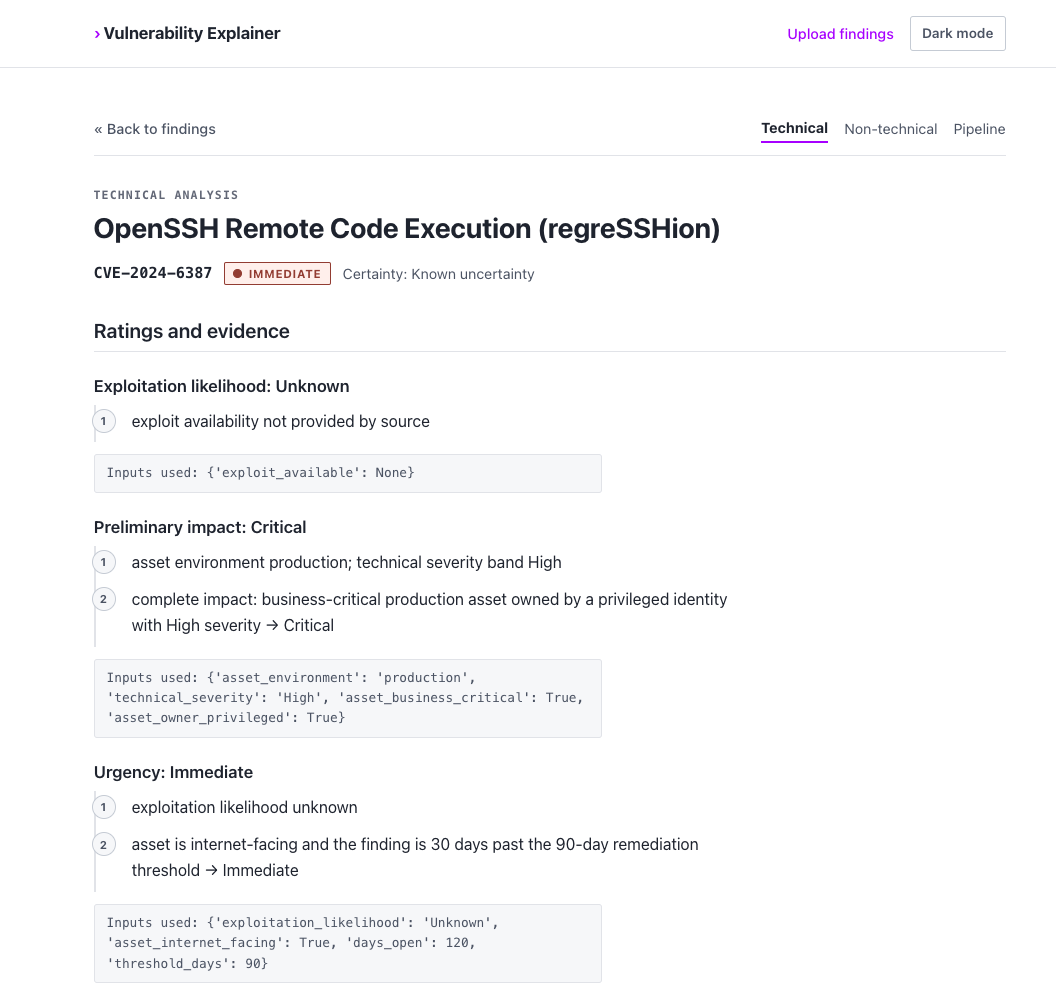
\includegraphics[width=\textwidth]{figures/output_technical_scenarioA.png}
\caption{Technical view output for Scenario A (clear critical finding).}
\label{fig:example-output-tech}
\end{figure}

\begin{figure}[h]
\centering
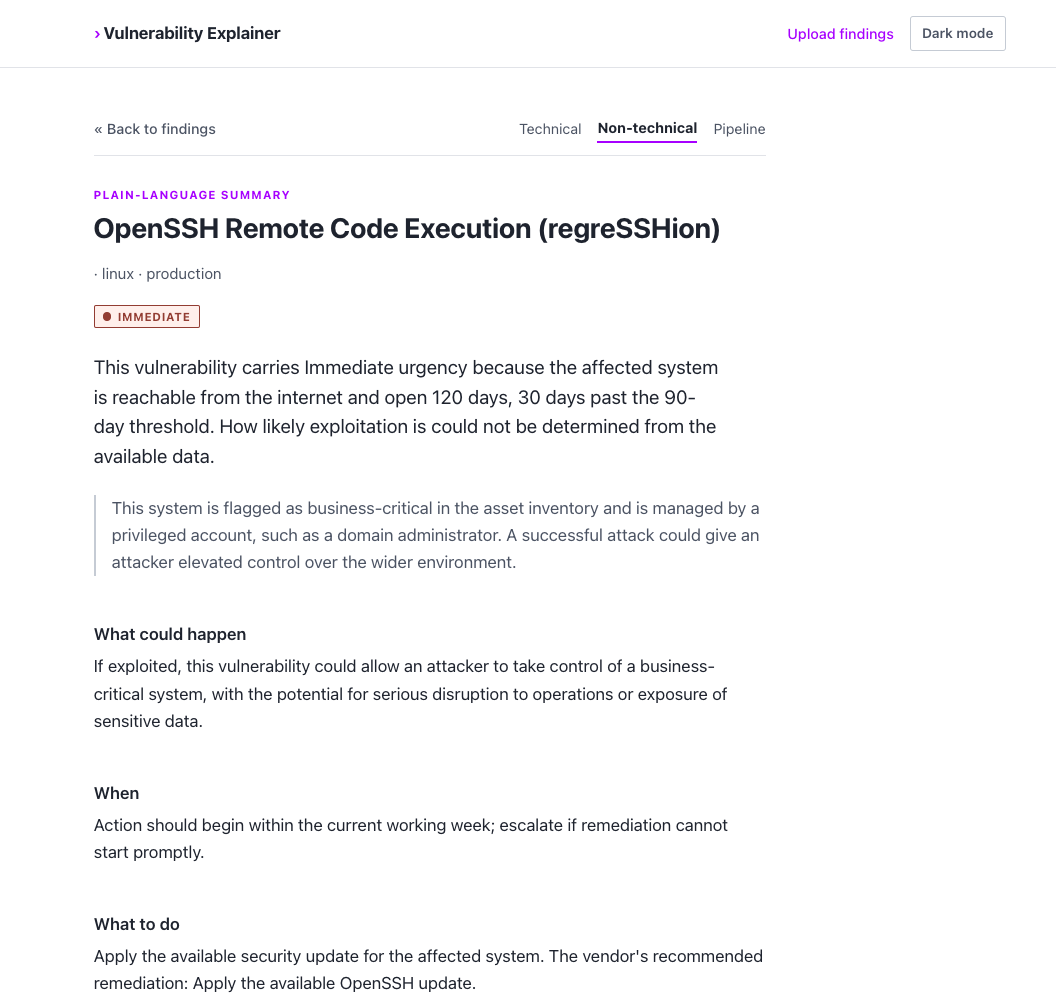
\includegraphics[width=\textwidth]{figures/output_nontechnical_scenarioA.png}
\caption{Non-technical view output for the same Scenario A finding.}
\label{fig:example-output-nontech}
\end{figure}